\documentclass[]{prezentare}
\graphicspath{{Imagini/}}

\title  {Operational monitoring of ATLAS TDAQ system}

\author [Cristian T\u al\u au]
        {\texorpdfstring
            {{\bf Author:} Cristian T\u al\u au \\ 
            {\bf Supervisors:} Prof. Roger Hersch, Dr. Wainer Vandelli}
            {Cristian Talau}  
      }
\institute {\texorpdfstring{\href{http://epfl.ch}
                {\' Ecole Polytechnique F\' ed\' erale de Lausanne - EPFL}}
                {\' Ecole Polytechnique F\' ed\' erale de Lausanne - EPFL}}
                
\titlegraphic {
  
\includegraphics[scale=0.2]{../Images/epfl_logo.png} 
  $\,$
  
\includegraphics[scale=0.05]{../Images/cern_logo.png}}


\begin{document}
\tikzstyle{every picture}+=[remember picture]
\tikzstyle{exec}=[rectangle,fill=black,minimum size=3pt,inner sep=0pt]
\begin{comment}
    \begin{frame}
        \titlepage
    \end{frame}

\begin{frame}
    \frametitle{Monitoring in the ATLAS TDAQ system}
    \begin{block}{Figures - global view}
    	\begin{itemize}
        	\item 15000 applications
        	\item running on 1500 nodes
            \item publish to 30 IS servers
      	\end{itemize}
  	\end{block}
    \begin{block}{Figures - single application}
    	\begin{itemize}
            \item publishes 5000 histograms
			\item with 500-1000 bins in average
            \item each histogram has a period between 5-120s
            \item 5-10 distinct periods in total
      	\end{itemize}
  	\end{block}
  	
\end{frame}

\begin{frame}[fragile]
     \frametitle{{\tt monsvc} Library}
     \begin{exampleblock}{Usage}
     	\begin{semiverbatim}
\alert<1>{ptr<TH1> phist = register("/DEBUG/event_size", &hist)}
\alert<2>{configure("/DEBUG/*", 30 * SEC, "DF")}
\alert<3>{start_publishing()}
...
\alert<4>{phist->update(event.size)}
...
stop_publishing()
        \end{semiverbatim}
	\end{exampleblock}
	\alt<2>{\begin{block}{Configuration}
	Provides a way to specify the publishing parameters associated with a given object.	
	\end{block}}{}
	\alt<3>{\begin{block}{Scheduling}
	Determines when to start publishing each histogram in each application.
	\end{block}}{}
	\alt<4>{\begin{block}{Synchronization}
	Ensures thread-safe access of the histogram for the application that updates it and the library thread which publishes it.
	\end{block}}{}
\end{frame}

%-----------------------------------------------------------------------------------

\begin{frame}
	\frametitle{Configuration}
	\begin{block}<1->{Challenge: Code size}
	\begin{description}
	\item [Problem]	Changing config. in a large codebase.
	\item [Solution] Store the config. in an external database.
	\end{description}
	\end{block}
	
	\begin{block}<2->{Challenge: Number of objects}
	\begin{description}
	\item [Problem] Specifying the config. for a large number of objects.
	\item [Solution] Use regex. to group object with similar configuration and to specify exceptions.
	\end{description}
	\end{block}
	
	\begin{block}<3->{Challenge: Multiple developers}
	\begin{description}
	\item [Problem] Apps are built from independently developed libs.
	\item [Solution] The config. is composed of rule bundles of the libs.
	\end{description}
	\end{block}
\end{frame}

%-----------------------------------------------------------------------------------

\begin{frame}[fragile]
	\frametitle{Synchronization}
	\begin{columns}
		\begin{column}{0.3\linewidth}
		
			\begin{block}{\tikz[baseline] \node (lt) {Library thread};}
				\begin{semiverbatim}
# lock:
\alert<2>{obj.lock()}

# unlock:
\alert<7>{with upd.lock: }
\alert<8>{  upd.exec()}
\alert<9>{  obj.unlock()}
				\end{semiverbatim}	
			\end{block}
		\end{column}

		\begin{column}{0.3\linewidth}
			\begin{tabular}{r l}
			{\tt obj} & 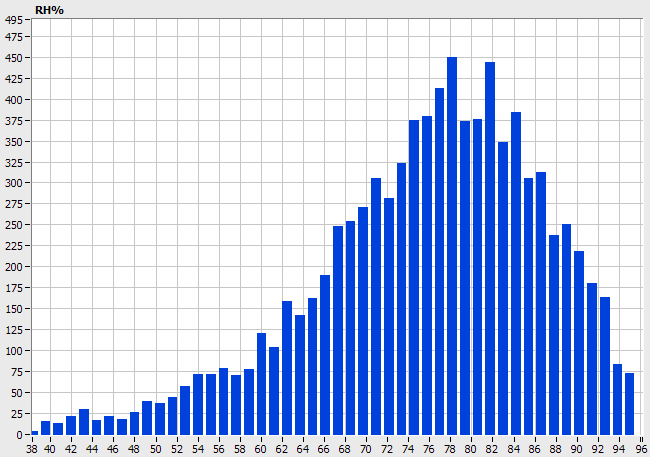
\includegraphics[scale=0.05]{../Images/histogram.png}
			\alt<2-9>{
			\begin{tikzpicture}[overlay]
				\node[yshift=5ex, xshift=-0.5ex] (objlock)
				  {
\includegraphics[scale=0.025]{../Images/lock.png}};
			\end{tikzpicture}
			}{} \\
			&\\
			{\tt upd} & \alt<6-8>{[(f,args)]}{[\, ]}
			\alt<3-14>{
			\begin{tikzpicture}[overlay]
				\node[yshift=1.75ex, xshift=-1ex] (updlock)
				  {
\includegraphics[scale=0.025]{../Images/lock.png}};
			\end{tikzpicture}
			}{} \\
			\end{tabular}	
		\end{column}
 		
		\begin{column}{0.4\linewidth}
			\begin{block}{\tikz[baseline] \node (mt) {Main thread};}
				\begin{semiverbatim}
# async(f, args):
\alert<3,10>{with upd.lock:}
\alert<4,11>{  if obj.try_lock():}
\alert<12>{    upd.exec()}
\alert<13>{    f(args)}
\alert<14>{    obj.unlock()}
\alert<5>{  else: }
\alert<6>{    upd.apnd(f, args)}
				\end{semiverbatim}
			\end{block}
		\end{column}
	\end{columns}

	\begin{tikzpicture}[overlay]
        \path<2-9>[->,thick] (objlock) edge [bend right] (lt);
        \path<3-6>[->,thick] (updlock) edge [bend left] (mt);
        \path<7-9>[->,thick] (updlock) edge [bend right] (lt);
        \path<10-14>[->,thick] (updlock) edge [bend left] (mt);
	\end{tikzpicture}

\end{frame}
%-----------------------------------------------------------------------------------
\begin{frame}
	\frametitle{Scheduling requirements}
	\begin{block}{Global}
		\begin{itemize}
			\item Minimize latency
			\item Minimize publishing skew
			\item Maximize throughput
		\end{itemize}
	\end{block}

	\begin{block}{Local}
		\begin{itemize}
			\item Minimize jitter
			\item Efficient reconfiguration
		\end{itemize}
	\end{block}
	
\end{frame}
%-----------------------------------------------------------------------------------
\begin{frame}
	\frametitle{Global vs. Local scheduling}
	\begin{block}{Time slots}
	\begin{itemize}
	\item Divide the time into equal length slots. 
	\item Slot length is configurable and we expect 1s = 30-100 slots.
	\end{itemize}	
	\end{block}

	\begin{definition}
	\emph{Local scheduling} decides which histogram(s) to publish in each time slot.
	\end{definition}

	\begin{definition}
	\emph{Global scheduling} decides when to start publishing the histogram(s) inside the assigned time slot.
	\end{definition}

\end{frame}

\begin{frame}
	\frametitle{Global scheduling}
	\begin{block}{Contradicting requirements}
	\begin{columns}[onlytextwidth]
		\begin{column}{0.5\textwidth}
		Minimize publishing skew
		
		\begin{tikzpicture}[node distance=1cm]
			\node (s1) at (0,0.5) [exec,label=west:{\scriptsize App. 3}] {};
            \node (e1) [exec,right of=s1] {};
            \draw [-,thick] (s1.east) -- (e1.west);

			\node (s2) at (0,1) [exec,label=west:{\scriptsize App. 2}] {};
            \node (e2) [exec,right of=s2] {};
            \draw [-,thick] (s2.east) -- (e2.west);

			\node (s3) at (0,1.5) [exec,label=west:{\scriptsize App. 1}] {};
            \node (e3) [exec,right of=s3] {};
            \draw [-,thick] (s3.east) -- (e3.west);

            \draw[-,dashed] (0,0.5) -- (3,0.5);
            \draw[-,dashed] (0,1.0) -- (3,1.0);
            \draw[-,dashed] (0,1.5) -- (3,1.5);
            \draw[-,dashed] (2,0.25) -- (2,2);
		\end{tikzpicture}
		\end{column}
		\begin{column}{0.5\textwidth}
		Minimize latency \& contention
		\begin{tikzpicture}[node distance=1cm]
			\node at (0,0.5) [label=west:{\scriptsize App. 3}] {};			
			\node (s1) at (0,0.5) [exec] {};
            \node (e1) [exec,right of=s1] {};
            \draw [-,thick] (s1.east) -- (e1.west);

			\node at (0,1) [label=west:{\scriptsize App. 2}] {};			
			\node (s2) at (1,1) [exec] {};
            \node (e2) [exec,right of=s2] {};
            \draw [-,thick] (s2.east) -- (e2.west);

			\node at (0,1.5) [label=west:{\scriptsize App. 1}] {};			
			\node (s3) at (2,1.5) [exec] {};
            \node (e3) [exec,right of=s3] {};

            \draw [-,thick] (s3.east) -- (e3.west);
            \draw[-,dashed] (0,0.5) -- (3,0.5);
            \draw[-,dashed] (0,1.0) -- (3,1.0);
            \draw[-,dashed] (0,1.5) -- (3,1.5);
            \draw[-,dashed] (2,0.25) -- (2,2);
		\end{tikzpicture}
		\end{column}
	\end{columns}
	\end{block}
	
	\begin{block}<2->{Solution}
	\begin{itemize}
	  \item Introduce a random delay of up to $f=75\%$ of the time slot. 
	  \item If the publishing takes longer, reduce the next interval(s).
	\end{itemize}
    \vspace{-5mm}
	\begin{center}
			\begin{tikzpicture}[node distance=1cm]
			\node at (0,0.5) [label=west:{\scriptsize App. 3}] {};			
			\node (s1) at (0.2,0.5) [exec] {};
            \node (e1) [exec,right of=s1] {};
            \draw [-,thick] (s1.east) -- (e1.west);

			\node at (0,1) [label=west:{\scriptsize App. 2}] {};			
			\node (s2) at (1.1,1) [exec] {};
            \node (e2) [exec,right of=s2] {};
            \draw [-,thick] (s2.east) -- (e2.west);

			\node at (0,1.5) [label=west:{\scriptsize App. 1}] {};			
			\node (s3) at (0.8,1.5) [exec] {};
            \node (e3) [exec,right of=s3] {};

            \draw [-,thick] (s3.east) -- (e3.west);
            \draw[-,dashed] (0,0.5) -- (3,0.5);
            \draw[-,dashed] (0,1.0) -- (3,1.0);
            \draw[-,dashed] (0,1.5) -- (3,1.5);
            \draw[-,dashed] (2,0.25) -- (2,2);
		\end{tikzpicture}
	\end{center}
	\end{block}
\end{frame}
%-----------------------------------------------------------------------------------
\begin{frame}
	\frametitle{Local scheduling}
	\begin{block}{Real-time system formulation}
	\begin{center}
	\begin{tabular}{r c l}
		task           & $\Longleftrightarrow$ & histogram \\
		job            & $\Longleftrightarrow$ & publishing a histogram \\
		execution time & $\Longleftrightarrow$ & latency \\
		period         & $\Longleftrightarrow$ & publishing interval \\	
		deadline       & $\Longleftrightarrow$ & jitter bound \\	
		CPU            & $\Longleftrightarrow$ & IS server \\
		utilization    & $\Longleftrightarrow$ & throughput \\
	\end{tabular}	
	\end{center}
	\end{block}

	\begin{block}<2->{Offset-free system}
	Our system permits different starting points for different tasks.
	\end{block}
\end{frame}
%-----------------------------------------------------------------------------------
\begin{frame}
	\frametitle{Local scheduling - Subperiod algorithm}
	\begin{exampleblock}{Two periods}
	Two histogram groups:
	\begin{itemize}
	\item 4=a+b+c histograms with period 15s
	\item 4=x+y histograms with period 10s
	\end{itemize}
	\vspace{-7.5mm}	
	\begin{center}
		\begin{tikzpicture}[node distance=0.75cm]
			\foreach \x in {0,1,2,3,4,5,6} {
				\node at (\x,0) [exec] (n0\x) {};
				\node at (\x,1) [exec] (n1\x) {};
			}
			
			\foreach \x/\la/\lb/\na/\nb in 
				{1/x/a/2/2, 2/y/b/2/1, 3/x/c/2/1, 4/y/a/2/2, 5/x/b/2/1, 6/y/c/2/1} {
				\node [text depth=0pt, text height=12pt, above left of=n1\x ,yshift=-7pt] {\alt<2>{\alert{\footnotesize \nb}}{\footnotesize \lb}};
				\node [text depth=0pt, text height=12pt, above left of=n0\x, yshift=-7pt] {\alt<2>{\alert{\footnotesize \na}}{\footnotesize \la}};
			}
			
%			\node at (-2,0) [text width=2.5cm] {x+y=4 histo. $\pi$=10s};
%			\node at (-2,1.5) [text width=2.5cm] {4=x+y histo. $\pi$=15s};
			
			% linii punctate
            \draw[-,dashed] (-0.5,0) -- (6.5,0);
            \draw[-,dashed] (-0.5,1) -- (6.5,1);
            
            % paranteze 
            \draw<1> [decorate, decoration={brace,amplitude=4pt,mirror,raise=5pt},xshift=0pt]
            (0,1) -- (1,1) node [black,midway,yshift=-14pt] {\footnotesize 5s};
            \draw<1> [decorate, decoration={brace,amplitude=4pt,mirror,raise=2pt},xshift=0pt]
            (0,1) -- (3,1) node [black,midway,yshift=-14pt] {\footnotesize 15s};
            \draw<1> [decorate, decoration={brace,amplitude=4pt,mirror,raise=2pt},xshift=0pt]
            (0,0) -- (2,0) node [black,midway,yshift=-11pt] {\footnotesize 10s};
            % paranteze 
            \draw<2> [decorate, decoration={brace,amplitude=4pt,mirror,raise=2pt},xshift=0pt]
            (0,1) -- (1,1) node [black,midway,yshift=-11pt] {\footnotesize 5s};
		\end{tikzpicture}
	\end{center}
	\end{exampleblock}

	\alt<1>{
	\begin{exampleblock}{Goal}
	  Minimize:
	  \vspace{-2.5mm}
	  \begin{equation*}
		  \max(x+a, y+b, x+c, \ldots) = \max(a, b, c) + \max(x, y)
	  \end{equation*}
	\end{exampleblock}
	}{
	\begin{exampleblock}<2>{Solution}
		We can (over-)approximate with  4 histograms and period 5s.
	\end{exampleblock}
	}
\end{frame}
%-----------------------------------------------------------------------------------
\begin{frame}
	\frametitle{Local scheduling - Subperiod algorithm}
	\begin{exampleblock}{Hierarchical approximation}
	
	\tikzstyle{leaf}=[rectangle,draw=black,very thick,fill=skyblue,minimum width=10pt,minimum height=5pt,inner sep=0pt]
	\tikzstyle{interns}=[rectangle,draw=black,very thick,fill=purple,minimum width=10pt,minimum height=5pt,inner sep=0pt]
	\tikzstyle{internl}=[rectangle,draw=black,very thick,fill=purple,minimum width=35pt,minimum height=15pt,inner sep=0pt]

	\begin{center}
	\begin{tikzpicture}
		\uncover<13->{\node [internl] (root) {4/1s};}
		\uncover<12->{\node 
			[internl,above left of=root,node distance=2cm,xshift=-1cm] (2s) {5/2s};}
		\uncover<8 ->{\node 
			[internl,above right of=root,node distance=2cm,xshift=1cm] (5s) {4/5s};}
		\uncover<4 ->{\node 
			[internl,above right of=5s,node distance=2cm] (15s) {4/15s};}
		\uncover<7 ->{\node [internl,above left of=5s,node distance=2cm] (10s) {4/10s};}
		\uncover<8 ->{\draw           (5s) -- (15s);}
		\uncover<13->{\draw (root) -- (5s);}
		\uncover<8 ->{\draw           (5s) -- (10s);}
		\uncover<13->{\draw (root) -- (2s);}
		
		
		\uncover<11->{\node [interns,above left of=2s,node distance=1cm] (2si1) {};}
		\uncover<10->{\node [interns,above right of=2s,node distance=1cm] (2si2) {};}
		\uncover<9 ->{\node [interns,above right of=2si2,node distance=0.5cm] (2si3) {};}
		\node [leaf,above left of=2si1,node distance=0.5cm] (2l1) {};
		\node [leaf,above right of=2si1,node distance=0.5cm] (2l2) {};
		\node [leaf,above left of=2si2,node distance=0.5cm] (2l3) {};
		\node [leaf,above left of=2si3,node distance=0.5cm] (2l4) {};
		\node [leaf,above right of=2si3,node distance=0.5cm] (2l5) {};
		\uncover<11->{\draw         (2si1) -- (2l1);}
		\uncover<12->{\draw (2s) -- (2si1);}
		\uncover<11->{\draw         (2si1) -- (2l2);}
		\uncover<10->{\draw         (2si2) -- (2l3);}
		\uncover<12->{\draw (2s) -- (2si2);}
		\uncover<9 ->{\draw                   (2si3) -- (2l4);}
		\uncover<10->{\draw         (2si2) -- (2si3);}
		\uncover<9 ->{\draw                   (2si3) -- (2l5);}
		
		
		\uncover<6- >{\node 
		  [interns,above left of=10s,node distance=1cm,xshift=0.25cm] (10si1){};}
		\uncover<5- >{\node [interns,above left of=10si1,node distance=0.5cm] (10si2) {};}
		\node [leaf,above left of=10si2,node distance=0.5cm] (10l1) {};
		\node [leaf,above right of=10si2,node distance=0.5cm] (10l2) {};
		\node [leaf,above right of=10si1,node distance=0.5cm] (10l3) {};
		\node [leaf,above right of=10s,node distance=1cm,xshift=-0.25cm] (10l4) {};	
		\uncover<5- >{\draw                     (10si2) -- (10l1);}
		\uncover<6- >{\draw          (10si1) -- (10si2);}
		\uncover<5- >{\draw                     (10si2) -- (10l2);}
		\uncover<7- >{\draw (10s) -- (10si1);}
		\uncover<6- >{\draw          (10si1) -- (10l3);}
		\uncover<7- >{\draw (10s) -- (10l4);}


		\uncover<2 ->{\node [interns,above left of=15s,node distance=1cm] (15si1) {};}
		\uncover<3 ->{\node [interns,above right of=15s,node distance=1cm] (15si2) {};}
		\node [leaf,above left of=15si1,node distance=0.5cm] (15l1) {};
		\node [leaf,above right of=15si1,node distance=0.5cm] (15l2) {};
		\node [leaf,above left of=15si2,node distance=0.5cm] (15l3) {};
		\node [leaf,above right of=15si2,node distance=0.5cm] (15l4) {};	
		\uncover<2- >{\draw          (15si1) -- (15l1);}
		\uncover<4 ->{\draw (15s) -- (15si1);}
		\uncover<2- >{\draw          (15si1) -- (15l2);}
		\uncover<3- >{\draw          (15si2) -- (15l3);}
		\uncover<4- >{\draw (15s) -- (15si2);}
		\uncover<3- >{\draw          (15si2) -- (15l4);}
	
		% acolade		
        \draw [decorate, decoration={brace,mirror,amplitude=10pt,raise=7pt}]
            (2l5.north east) -- +(-3cm,0)
            node [black,midway,yshift=25pt] {2s};

        \draw [decorate, decoration={brace,amplitude=10pt,raise=7pt}]
            (10l1.north west) -- +(2.25cm,0)
            node [black,midway,yshift=25pt] {10s};

        \draw [decorate, decoration={brace,amplitude=10pt,raise=7pt}]
            (15l1.north west) -- +(2.6cm,0)
            node [black,midway,yshift=25pt] {15s};
            
        % offset propagation: starting from 14
        \node [right of=root,node distance=2.25cm,text width=3cm] 
        	{\alt<14>
        		{\tiny \{0, .25, .5, .75\}}
        		{\alt<15-16>
        			{\tiny \{0, .25, .5\}}
        			{\alt<17->
        				{\tiny\{\}}
        				{}
        			}
        		}
        	};
        \node [right of=2s,node distance=2.25cm,text width=3cm]  (o1)
        	{\alt<17>
        		{\tiny \{0, .25, .5\}}
        		{\alt<18>
        			{\tiny \{0, .25, .5, 1, 1.25, 1.5\}}
        			{\alt<19>
        				{\tiny \{.5, 1, 1.25, 1.5\}}
        				{\alt<20->
        					{\tiny \{1.5\}}
        					{}
        				}
        			}
        		}
        	};

        \node [right of=5s,node distance=2.25cm,text width=3cm] (o2)
        	{\alt<15>
        		{\tiny \{.75\}}
        		{\alt<16-26>
        			{\tiny \{.75, 1.75, $\ldots$\}}
        			{\alt<27->
        				{\tiny \{4.75\}}
        				{}
        			} 
        		}
        	};

		\node [left of=2si1,,node distance=.75cm,text width=1cm] 
			{\hfill \alt<19-20>
				{\tiny \{0, .25\}}
				{\alt<21>
					{\tiny \{.25\}}
					{\alt<22->
						{\tiny \{\}}
						{}
					}
				}
			};
			
		\node [right of=2si2,node distance=1.5cm,text width=2cm] 
			{\alt<20-22>
				{\tiny \{.5, 1, 1.25\}}
				{\alt<23>
					{\tiny \{1, 1.25\}}
					{\alt<24->
						{\tiny \{\}}
						{}
					}
				}
			};

        \uncover<21- >{\node [above of=2l1,node distance=.25cm] {\tiny \bf 0};}
        \uncover<22- >{\node [above of=2l2,node distance=.25cm] {\tiny \bf .25};}       
        \uncover<23- >{\node [above of=2l3,node distance=.25cm] {\tiny \bf .5};}
        
        \node [right of=2si3,node distance=.7cm] 
        	{\alt<24>
        		{\tiny \{1, 1.25\}}
        		{\alt<25>
        			{\tiny \{1.25\}}
        			{\alt<26->
        				{\tiny \{\}}
        				{}
        			}
        		}
        	};

        \uncover<25- >{\node [above of=2l4,node distance=.25cm] {\tiny \bf 1};}
        \uncover<26- >{\node [above of=2l5,node distance=.25cm] {\tiny \bf 1.25};}
        
        \uncover<27 ->{
	        \node [above of=10l1,node distance=.25cm] {\tiny \bf .75};
	        \node [above of=10l2,node distance=.25cm] {\tiny \bf 1.75};
	        \node [above of=10l3,node distance=.25cm,xshift=0.1cm] {\tiny \bf 5.75};
	        \node [above of=10l4,node distance=.25cm] {\tiny \bf 6.75};
	        
	        \node [above of=15l1,node distance=.25cm] {\tiny \bf 2.75};
	        \node [above of=15l2,node distance=.25cm] {\tiny \bf 3.75};
	        \node [above of=15l3,node distance=.25cm] {\tiny \bf 7.75};
	        \node [above of=15l4,node distance=.25cm] {\tiny \bf 12.75};
	        
	        \node [right of=10s,node distance=2cm,text width=2.5cm] {\tiny \{\}};
	        \node [right of=15s,node distance=1.5cm,text width=1.5cm] 
	        	(o3) {\tiny \{8.75, 13.75\}};
        }
        
        \uncover<28- >{
        	\node at (o1.west) 
        		[shape=rectangle,draw=red,very thick,inner sep=0,minimum width=.6cm,minimum height=0.4cm,xshift=0.4cm] (or1) {};
        	\node at (o2.west) 
        		[shape=rectangle,draw=red,very thick,inner sep=0,minimum width=.7cm,minimum height=0.4cm,xshift=0.45cm] (or2) {};
        	\node at (o3.west) 
	        	[shape=rectangle,draw=red,very thick,inner sep=0,minimum width=1.4cm,minimum height=0.4cm,xshift=.8cm] (or3) {};
	        	
        	\node [right of=root,node distance=2cm,text=red] (unused1)
        		{$\frac 1 2$ + };
        	\node [right of=unused1,node distance=.75cm,text=red] (unused2)       		
				{$\frac 1 5$ + }; 
        	\node [right of=unused2,node distance=.6cm,text=red] (unused3)
				{$\frac 2 {15} $};
        	\node [right of=unused3,node distance=1.5cm,text=red] (unused4)
				{unused slots/s};
				
	        \path[->,thick,draw=red] (unused1) edge [bend right] (or1);
	        \path[->,thick,draw=red] (unused2) edge [bend left] (or2);
	        \path[->,thick,draw=red] (unused3) edge [bend right] (or3);        	
        }
        \end{tikzpicture}
	\end{center}	
	\end{exampleblock}
\end{frame}
\end{comment}
%-----------------------------------------------------------------------------------%
\begin{frame}
	\frametitle{Local scheduling}
	\begin{block}{Subperiod algorithm - results}
	
	\end{block}
\end{frame}
%-----------------------------------------------------------------------------------
\begin{comment}
\begin{frame}
	\frametitle{Conclusions}

	\begin{block}{Contributions}
	\begin{itemize}
	\item Configuration specification.
	\item Subperiod scheduling algorithm.
	\item Policy-based synchronization including asynchronous updates policy.
	\end{itemize}		
	\end{block}

	\begin{block}{Possible further improvements}
	\begin{itemize}
	\item Atomic and synchronized configuration of multiple applications.
	\item Improve the scheduling algorithm to assign multiple consecutive slots to a single large histogram.
	\end{itemize}		
	\end{block}

\end{frame}
%-----------------------------------------------------------------------------------
    \begin{frame}
    \setbeamercolor{qa}{fg=block title.fg,bg=block title.bg} %structure.fg

    \begin{beamercolorbox}[rounded=true,shadow=true]{qa}
    \begin{center}
        {\Huge \textbf{Questions?}}
    \end{center}
    \end{beamercolorbox}
    \end{frame}
\end{comment}
\end{document}
